%\documentclass[landscape,pagesize,DIV=14]{scrartcl}
\documentclass[border=2mm]{standalone}

\usepackage[utf8]{inputenc}
\usepackage[T1]{fontenc}

\usepackage{amsmath}

\usepackage{tikz}
\usetikzlibrary{graphs}%,graphdrawing}
\usetikzlibrary{positioning}
\usetikzlibrary{calc}

\newcommand{\code}[1]{\texttt{#1}}
\newcommand{\Owns}[1]{{\color{red}#1}}

\definecolor{mycontour}{HTML}{43709A}
\definecolor{myfill}{HTML}{E2EBF2}
\newlength\separation
\setlength{\separation}{1ex}

\begin{document}

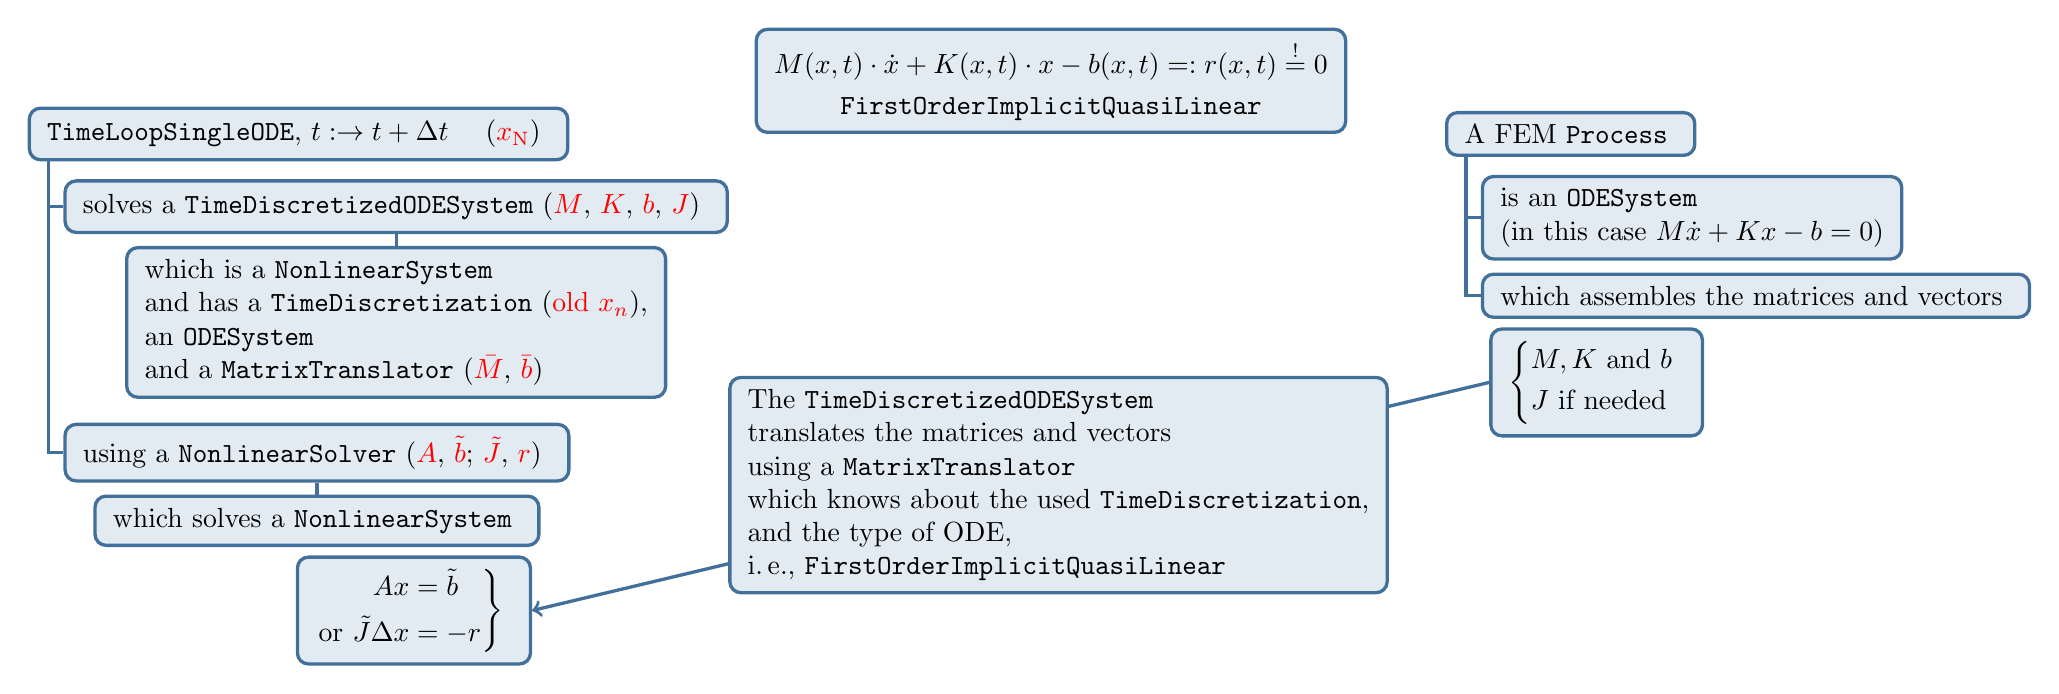
\begin{tikzpicture}[
    very thick,
    align=left, anchor=west,
    node distance=\separation,
    color=mycontour,
    text=black,
    every node/.style={
      inner ysep=\separation,
      inner xsep=1.5\separation,
      rectangle,
      rounded corners,
      draw=mycontour,
      fill=myfill
    }
]
  \node (timeloop) at (0,0) {
    \code{TimeLoopSingleODE}, $t :\to t + \Delta t$
    \quad (\Owns{$x_\text{N}$})
  };
  \node (tdodesys) [below right=1.5\separation and 3\separation of timeloop.south west, anchor=north west] {
    solves a \code{TimeDiscretizedODESystem}
    (\Owns{$M$}, \Owns{$K$}, \Owns{$b$}, \Owns{$J$})
  };
  %\node (tdodesysDetail) [below right=of tdodesys.south west] {
  \node (tdodesysDetail) [below=of tdodesys] {
    which is a \code{NonlinearSystem}
    \\ and has a \code{TimeDiscretization} (\Owns{old $x_n$}),
    \\ an \code{ODESystem}
    \\ and a \code{MatrixTranslator} (\Owns{$\bar M$}, \Owns{$\bar b$})
  };
  \path let \p1=(tdodesys.west), \p2=(tdodesysDetail.south)
  in node (nlsolver) [anchor=north west] at (\x1,\y2-2\separation) {
    using a \code{NonlinearSolver} (\Owns{$A$}, \Owns{$\tilde b$}; \Owns{$\tilde J$}, \Owns{$r$})
  };
  % \node (nlsolverDetail) [below right=of nlsolver.south west] {
  \node (nlsolverDetail) [below=of nlsolver] {
    which solves a \code{NonlinearSystem}
  };
  \node (nlsolverDetail2) [below left=of nlsolverDetail.south east, anchor=north east] {
    {$
      \left.
      \begin{aligned}
        Ax &= \tilde b \\
        \text{or } \tilde J \Delta x &= -r
      \end{aligned}
      \right\}
    $}
  };

  \node (process) at (18, 0) { A FEM \code{Process} };
  \node (processDetail) [below right=1.5\separation and 3\separation of process.south west] {
    is an \code{ODESystem} \\
    (in this case $M\dot x + Kx - b = 0$)
  };
  \node (assembly) [below=of processDetail.south west, anchor=north west] {
    which assembles the matrices and vectors
  };
  \node (assembly2) [below right=of assembly.south west, anchor=north west] {
    $\left\{
      \begin{aligned}
        &M, K \text{ and } b \\
        &J \text{ if needed}
      \end{aligned}
      \right.$
  };

  \path[draw=none] (timeloop.east) -- node [pos=0.55, above, anchor=south, align=center] {
    $M(x,t) \cdot \dot x + K(x,t) \cdot x - b(x,t) =: r(x,t) \stackrel!= 0$ \\[1mm]
    \code{FirstOrderImplicitQuasiLinear}
  } (process.west);

  \draw let \p1=(timeloop.south west) in (\x1+1.75\separation,\y1) |- (tdodesys);
  \draw let \p1=(timeloop.south west) in (\x1+1.75\separation,\y1) |- (nlsolver);

  \draw let \p1=(process.south west) in (\x1+1.75\separation,\y1) |- (processDetail);
  \draw let \p1=(process.south west) in (\x1+1.75\separation,\y1) |- (assembly);

  \draw (tdodesysDetail) -- (tdodesys);
  \draw (nlsolver) -- (nlsolverDetail);

  \draw[<-] (nlsolverDetail2.east) --
  node [pos=0.55, anchor=center] {
    The \code{TimeDiscretizedODESystem} \\
    translates the matrices and vectors \\
    using a \code{MatrixTranslator} \\
    which knows about the used \code{TimeDiscretization}, \\
    and the type of ODE, \\
    i.\,e., \code{FirstOrderImplicitQuasiLinear}
  } (assembly2.west);

\end{tikzpicture}

\end{document}
